\documentclass[11pt]{article}
\usepackage[T1]{fontenc}
\usepackage{lmodern,amsmath,amssymb,amsthm,mathtools,booktabs,graphicx}
\usepackage[letterpaper,left=.94in,right=.94in,top=.84in,bottom=.88in]{geometry}
\usepackage{microtype,xcolor,fancyhdr,titlesec}
\usepackage[hyphens]{url}
\usepackage[colorlinks=true,linkcolor=teal!55!black,urlcolor=teal!55!black,citecolor=teal!55!black]{hyperref}
\definecolor{ink}{HTML}{20394B}\definecolor{accent}{HTML}{076F70}
\titleformat{\section}{\large\bfseries\sffamily\color{ink}}{\thesection}{.72em}{}
\titleformat{\subsection}{\normalsize\bfseries\sffamily\color{accent}}{\thesubsection}{.6em}{}
\titlespacing*{\section}{0pt}{2.5ex plus .6ex}{1.0ex}
\titlespacing*{\subsection}{0pt}{1.9ex plus .5ex}{.6ex}
\newtheorem{theorem}{Theorem}[section]
\setlength{\parindent}{1.1em}\setlength{\emergencystretch}{2em}
\pagestyle{fancy}\fancyhf{}\fancyhead[L]{\footnotesize\sffamily\color{ink}Torsion selection and signed zero data}
\fancyhead[R]{\footnotesize\sffamily\color{ink}Research note}\fancyfoot[C]{\small\thepage}
\setlength{\headheight}{14pt}\renewcommand{\headrulewidth}{.25pt}
\hypersetup{pdftitle={How far must a torsion selector search?},pdfsubject={Three transfers from the Lean proof of Dirichlet GRH}}
\newcommand{\ghlink}[2]{\href{https://github.com/lsernau/grh-lean/blob/72fead102f663d5c7a407964a13dc0cf9d977207/#1}{#2}}
\begin{document}\raggedbottom
\thispagestyle{plain}
{\small\sffamily\color{accent}NUMBER THEORY\hfill 25 NOVEMBER 2026}\par\vspace{12pt}
{\noindent\fontsize{24}{28}\selectfont\bfseries\sffamily\color{ink}How far must a torsion selector search?\par}
\vspace{4pt}
{\noindent\large\sffamily Sharp bounds and two analytic transfers from the Lean proof of Dirichlet GRH\par}
\vspace{9pt}\noindent{\color{accent}\rule{\linewidth}{.7pt}}\par\vspace{5pt}
\noindent A quantitative question in an earlier ProveIt report asks whether one can efficiently choose a root of unity at which each of many $p$-adic polynomials keeps its valuation close to a known value. With arbitrary integral algebraic coefficients and a bound only on the total budget, the answer is negative. We give the exact cost of defeating all choices up to a prescribed order. It changes sharply at budget $p/(p-1)$: above that value, the worst necessary order exponent is exponential in inverse tolerance. At $p=2$, budget $3$ and tolerance $1/8$, the exact worst first successful exponent is $372$. With coefficients in $\mathbb Q_2$ it is $4$.

\medskip\noindent Two other parts of the proof lead to different conclusions. A finite list of signed zero multiplicities with certified precision suffices to recover the hidden modulus and quadratic twist in its arithmetic parameter range. For a non-CM elliptic curve, one optimized nonnegative polynomial in the local traces gives a single fourth-power sampling criterion for GRH for the first $2d$ symmetric powers. Its required arithmetic estimate remains open.

\section{Which parts of the Lean proof transfer?}
The readable and compact editions of \cite{repo} prove the classical RH and GRH for Dirichlet characters of every positive modulus, including imprimitive characters. The exported half-plane nonvanishing theorem excludes the principal pole. We inspected the readable source at commit \texttt{72fead1}. Its README records the kernel and external checks with Lean 4.35.0 and the pinned Mathlib revision. The arguments in this report are mathematical proofs with computational checks of selected consequences. We did not rerun the upstream build or formalize these extensions.

Three source declarations explain the choices of problems:
\begin{itemize}\setlength{\itemsep}{2pt}
\item \ghlink{grh/src/New/Congruences/Selmer/RootsOfUnity.lean}{\texttt{exists\_rootOfUnity\_eval\_le\_gaussVal\_add}} selects a primitive root of some order $p^h$ by summing a valuation budget over the distinct radii. This feeds the Selmer twisting argument in the determinant lower bound. Sections 2--4 determine exactly what this general selection principle costs in one variable.
\item \ghlink{grh/src/New/Reduction/Zeros/PrimeError.lean}{\texttt{isPolar\_primeRemainder}} identifies the Mellin residues of a weighted prime sum as signed differences of zero orders. At $s=1/2+i\gamma$ the residue is $m(\gamma)/(1/4+\gamma^2)$. Section~\ref{sec:inverse} uses the numerator, with common zeros already combined.
\item The \ghlink{grh/src/New/Reduction/Zeros/Criterion.lean}{one-sided zero criterion} chooses a twist depending on a hypothetical zero and uses the sign of real residues to rule it out. Section~\ref{sec:sym} arranges the sign for symmetric powers by character coefficients and uses convexity to pass from fourth powers to all cutoffs.
\end{itemize}
\noindent In the source, short integral forms, a spanning estimate and a determinant lower bound give the \ghlink{grh/src/New/Reduction/MainInequality.lean}{main inequality} after the common height term cancels. This supplies the prime-sum upper bound for congruence and quadratic-character weights. Its inputs are specific to those weights. Section~\ref{sec:sym} quantifies the obstruction to reproducing elliptic trace weights by a fixed modulus.

\newpage\section{The cost of simultaneous torsion selection}

Let $v$ be the valuation on $\overline{\mathbb Q}_p$ with $v(p)=1$ and $v(0)=+\infty$. Write $\mathcal U_h$ for the roots of exact order $p^h$, $e_h=(p-1)p^{h-1}$, and $r_h=1/e_h$. For an integral polynomial $g=\sum_j a_jT^j$, its Gauss valuation at radius parameter $r$ is
\[
 G_r(g)=\min_j\{v(a_j)+jr\}.
\]
Thus $v(g(y))\ge G_r(g)$ for $v(y)=r$. The root of unity in the source selector is evaluated in the coordinate $T=\zeta-1$.

\paragraph{The question.}
The closing research question (ii) of the incoming \emph{Quantitative twists} manuscript \cite{priortorsion} asks whether a bound on the shell exponent $H$ can be polynomial in the total budget and inverse tolerance, uniformly in degrees and packet size, while controlling total positive excess. In the earlier manuscript on torsion selection the relevant one-variable assertion has the following parameters. Each polynomial $g_i$ has an integral algebraic coefficient set and a witness $x_i$ with $v(x_i)\ge\rho$. Set $t_i=v(g_i(x_i))<\infty$ and assume $\sum_i t_i\le B$. One seeks $h\le H$ with $r_h\le\rho$ and $\zeta\in\mathcal U_h$ such that
\[
 \sum_i \big(v(g_i(\zeta-1))-t_i\big)_+\le\epsilon,
 \qquad (u)_+=\max(u,0).
\]
The argument from the source gives a cardinality-independent sufficient bound exponential in $(B+1)/\epsilon$ for $0<\epsilon<1$, with fixed depth and dimension. The quantitative twists manuscript gives a polynomial bound for a fixed finite packet with an exponent that depends on the number of constraints, for comparison to the fixed-depth Gauss valuations. Its example that vanishes on every point of $H$ shells costs budget $H$. Controlling positive excess permits cheaper obstructions.

\paragraph{Theorem (exponential lower bound).}
Fix $p=2$, $\rho=1$ and $0<\epsilon<1$. For every integer $H\ge1$ there are $H$ monic integral polynomials, all defined over $\mathbb Q_2(\zeta_{2^H})$, with the same witness $x_i=0$ and total budget
\[
 B_H\le 2+4\epsilon\sum_{j=1}^{H-1}\frac1j .
\]
For every $1\le h\le H$ and every $\zeta\in\mathcal U_h$, at least one of the individual excesses exceeds $\epsilon$. In particular for $0<\epsilon\le1/8$ and $B=3$ no selector can guarantee success by shell
\[
 H=\left\lfloor\exp\!\left(\frac{1}{8\epsilon}\right)\right\rfloor.
\]
Together with the harmonic upper bound this gives $\exp(\Theta(1/\epsilon))$ for the worst-case first successful shell exponent at fixed $B=3$. The order of the root itself is $2^h$.

\paragraph{Proof.}
Fix a primitive $2^h$-th root $z_h$ in each shell. For $1\le k\le h$, choose the transversal $A_k=\{1,3,\ldots,2^k-1\}$ of odd residue classes modulo $2^k$ and put
\[
 g_{h,k}(T)=\prod_{a\in A_k}\big(T-(z_h^a-1)\big),
 \qquad t_{h,k}=2^{k-h}.
\]
All $2^{k-1}$ roots have valuation $r_h=2^{1-h}$. Multiplicativity of Gauss valuations gives
\[
 v(g_{h,k}(0))=G_1(g_{h,k})=G_{r_h}(g_{h,k})=t_{h,k}.
\]
The identity $v(z_h^u-1)=2^{v_2(u)}/2^{h-1}$ for $2^h\nmid u$ follows from the order of $z_h^u$. Indeed, the primitive $2^m$-th roots give conjugate differences from $1$, whose product up to sign is $\Phi_{2^m}(1)=2$.

For any odd $b$ and each $1\le j<k$, exactly $2^{k-j-1}$ members of $A_k$ satisfy $v_2(a-b)=j$. These contribute $t_{h,k}$ to $v(g_{h,k}(z_h^b-1))$ for each such $j$. The one remaining $a$ agrees with $b$ modulo $2^k$. Its factor has valuation at least $2^k/2^{h-1}=2t_{h,k}$, with $+\infty$ allowed when the factor vanishes. Consequently
\[
 v\big(g_{h,k}(z_h^b-1)\big)-t_{h,k}\ \ge\ k\,t_{h,k}.
\]
When $k<h$ equality is attained at $b=1+2^k$. When $k=h$ every evaluation vanishes. The amplification by $k$ comes from the full set of nested congruence conditions on $a-b$.

For shell $h$ choose the least $k=k(h)\in\{1,\ldots,h\}$ such that $k2^{k-h}>\epsilon$. This exists because the expression at $k=h$ is $h$. Use the polynomial $g_{h,k(h)}$ as the $h$-th constraint. The preceding inequality blocks the entire shell. To sum the costs, the terms with $k(h)=1$ cost at most $\sum_{h\ge1}2^{1-h}=2$. When $k(h)=k\ge2$, minimality gives
\[
 2^{k-h}\le\frac{2\epsilon}{k-1}.
\]
With $k$ fixed these terms are distinct powers of $2$ and their sum is at most twice the largest. Summing over $k=2,\ldots,H$ yields the asserted budget. Finally $\sum_{j=1}^{H-1}j^{-1}\le1+\log H$, so the displayed exponential choice of $H$ costs at most $2+4\epsilon+1/2\le3$.\hfill$\square$

\paragraph{A single polynomial for the moving baseline.}
Set $P=\prod_{h=1}^H g_{h,k(h)}$. Then $G_1(P)=B_H$. At each primitive point of shell $h$,
\[
 v(P(\zeta-1))-G_{r_h}(P)>\epsilon.
\]
Indeed every factor has nonnegative excess over its own $G_{r_h}$, and the shell's designated factor has excess greater than $\epsilon$. This shows exponential sharpness in inverse tolerance for the source's stronger one-polynomial comparison to the moving Gauss valuation. Replacing that baseline by $G_1(P)$ can absorb an individual loss through savings on the other factors. This distinction accounts for the polynomial fixed-packet result in the earlier report.

\paragraph{What bounded ramification buys.}
Let $K/\mathbb Q_p$ be finite with absolute ramification index $e$. Suppose all $g_i$ are integral polynomials over $K$. Among the admissible shells $r_h\le\rho$, at most $\lfloor eB\rfloor$ contain a root valuation of any $g_i$ when $\sum_i G_\rho(g_i)\le B$. On every other admissible shell, \emph{all} primitive points simultaneously satisfy $v(g_i(\zeta-1))=G_{r_h}(g_i)\le G_\rho(g_i)$. Thus $\lfloor eB\rfloor+1$ consecutive admissible shells guarantee a shell of zero positive excess. The witness-budget version follows from $G_\rho(g_i)\le t_i$.

To see this, let $m_{ih}$ count the roots of $g_i$ of valuation $r_h$ with multiplicity. Their multiset is stable under the absolute Galois group of $K$. When $m_{ih}>0$ their product belongs to $K^\times$ and $m_{ih}r_h\ge 1/e$. Factorization of $g_i$ into linear factors gives
\[
 \sum_{h:r_h\le\rho} m_{ih}r_h\le G_\rho(g_i)-G_0(g_i)\le G_\rho(g_i).
\]
In fact a root of valuation $w$ contributes $\min(w,\rho)-\min(w,0)$ to the difference, a nonnegative amount. This argument includes roots at zero by the convention $w=+\infty$. Summation proves the exceptional-shell count. On a shell devoid of roots of matching valuation, the ultrametric inequality gives equality with the Gauss valuation in each linear factor. The counterexamples above use fields of growing ramification and freely chosen algebraic integral packets. Any application to narrower arithmetic families must separately determine which coefficient fields and polynomial packets can actually occur.

\section{The exact minimum budget for a counterexample}
\label{sec:exact}
Fix any prime $p$, depth $\rho=1$, and tolerance $\epsilon\ge0$. A family
\emph{blocks} the first $H$ shells if every allowed root of unity in those shells
has total positive excess strictly greater than $\epsilon$. Write
$C_p(\epsilon,H)$ for the least witness budget of such a family, allowing
arbitrarily many integral polynomials of arbitrary degrees over
$\overline{\mathbb Q}_p$. The minimum is attained. The following formula
computes it without searching over polynomials or coefficient fields.

\begin{theorem}\label{th:cost}
With $e_j=\varphi(p^j)$ define
\[
 U_h(m)=
 \begin{cases}
 \displaystyle\frac{1}{e_h}\sum_{j=1}^{h-1}e_j
                  \left\lfloor\frac{m}{e_j}\right\rfloor,&0\le m<e_h,\\[5pt]
 +\infty,& m\ge e_h .
 \end{cases}
\]
Let $m_h$ be the least nonnegative integer with $U_h(m_h)>\epsilon$. Then
\[
 \boxed{\displaystyle C_p(\epsilon,H)=\sum_{h=1}^H\frac{m_h}{e_h}.}
\]
Thus $B<C_p(\epsilon,H)$ guarantees success somewhere in shells $1$ through $H$.
At equality an explicit counterexample already exists with every witness at zero.
The statement also holds for a single polynomial if the excess in shell $h$ is
measured over its moving Gauss valuation $G_{r_h}$ and its budget is $G_1$.
\end{theorem}

\subsection*{A single shell}
Set $z_a=\xi^a-1$ for a fixed primitive $p^h$-th root $\xi$ and let $a$ run through
the units modulo $p^h$. Given $m$ algebraic roots $\alpha$ of valuation $r_h$,
counted with multiplicity, consider
\[
 \min_{a}\sum_\alpha \big(v(z_a-\alpha)-r_h\big).
\]
Its largest possible value is $U_h(m)$. To see the upper bound, replace each
$\alpha$ by a $z_b$ maximizing $v(z_b-\alpha)$ on this finite set.
For every $a$ the ultrametric inequality gives
$v(z_a-z_b)\ge\min\{v(z_a-\alpha),v(z_b-\alpha)\}=v(z_a-\alpha)$.
This replacement can only raise the minimum. We may therefore reason about a
multiset of $m$ unit residues $b$.

For a given $a$ write $N_j(a)$ for the number of these residues congruent to $a$
modulo $p^j$. If $a$ itself is unoccupied, the order of $\xi^{a-b}$ gives
\[
 v(z_a-z_b)=r_h p^{v_p(a-b)},\qquad
 \sum_b(v(z_a-z_b)-r_h)=r_h\sum_{j=1}^{h-1} e_j N_j(a).
\]
The second equality expands $p^t-1=\sum_{j=1}^t(p-1)p^{j-1}$.
Choose a least occupied unit class modulo $p$, then a least occupied child
modulo $p^2$, and continue. The first choice has at most $\lfloor m/(p-1)\rfloor$
occupants, and at each subsequent step one divides by $p$ and rounds down.
Consequently $N_j(a)\le\lfloor m/e_j\rfloor$ at every depth. If $m<e_h$, the
terminal residue is unoccupied. This proves the upper bound simultaneously at
all depths.

For the reverse bound, place the roots at the first $m$ positive unit exponents
in increasing order, omitting multiples of $p$. In every block of $e_j$
successive unit exponents, each unit class modulo $p^j$ occurs once. Thus every
$N_j(a)\ge\lfloor m/e_j\rfloor$. Occupied leaves give infinite valuation and
the other leaves give at least the required sum. For $m\ge e_h$, putting a root
at every leaf makes the minimum infinite. This includes the shell of order two
and the case $m=0$ by the empty-sum convention. The one-shell argument is a
cyclotomic instance of the fixed-divisor extremal principle underlying
Bhargava's $P$-orderings \cite{bhargava}. The global budget is a separate constraint.

\subsection*{Passing from one shell to every shell}
For a general family, take all roots of all the $g_i$, with multiplicities, and
let $M_h$ count the ones with valuation $r_h$. Factorization, or
multiplicativity of the Gauss valuation, yields
\[
 \sum_{h=1}^H M_h r_h\ \le\ \sum_i\big(G_1(g_i)-G_0(g_i)\big)
 \ \le\ \sum_i v(g_i(x_i)).
\]
In fact a root of valuation $w$ contributes $\min(1,w)-\min(0,w)$ to the
middle expression, which also handles roots of negative valuation, and
all $G_0(g_i)$ are nonnegative. For a primitive point in shell $h$ we have
$t_i\ge G_1(g_i)\ge G_{r_h}(g_i)$. The total positive excess is bounded by
$\sum_i (v(g_i(z_a))-G_{r_h}(g_i))$. In that sum every root with valuation
different from $r_h$ contributes zero, by the strict ultrametric equality.
The single-shell upper bound shows that blocking requires $M_h\ge m_h$.
Summing the charges proves the lower bound on $C_p$.

For equality, use one monic polynomial per shell, with roots at the first
$m_h$ ordered unit exponents as above. Its value at zero has valuation exactly
$m_hr_h$. On its designated shell its excess is at least $U_h(m_h)>\epsilon$.
The positive part prevents any saving from the other polynomials from canceling
this excess. All coefficients lie in $\mathbb Q_p(\zeta_{p^H})$. Multiplying
the polynomials gives the corresponding attainment for the moving Gauss
valuation, because its excess is additive and each summand is nonnegative.
\hfill$\square$

\paragraph{An exact contrasting case.}
For coefficients in a finite unramified extension of $\mathbb Q_p$,
the bound in the preceding section guarantees zero excess within the first
$\lfloor B\rfloor+1$ shells. It is optimal for every finite tolerance.
Indeed $\Phi_{p^h}(1+T)$ vanishes throughout shell $h$ and has value
$p$ at zero. Taking one such polynomial per shell costs exactly $H$ for $H$
shells. For unrestricted algebraic coefficients, subdividing the cost within
one shell is precisely what the floor sums measure.

\section{The sharp exponential rate and the critical budget}

The exact shell costs reveal a transition in the dependence on the tolerance. In this section $p$ is fixed, $\rho=1$, and $C_p(\epsilon,H)$ denotes the least total witness budget that can block all shells $1,\ldots,H$ with total positive excess strictly greater than $\epsilon$. Write $B_*=p/(p-1)$ and let $N_p(B,\epsilon)$ denote the worst possible first successful shell exponent over packets of budget at most $B$. Equivalently, $N_p$ is one plus the largest blocked initial horizon, with horizon zero always affordable.

\paragraph{Theorem.}
For every fixed $c>0$,
\[
 \lim_{\epsilon\downarrow0} C_p\!\left(\epsilon,\lfloor\exp(c/\epsilon)\rfloor\right)=B_*+c.
\]
Consequently, for every fixed $B>B_*$,
\[
 \boxed{\displaystyle\lim_{\epsilon\downarrow0}\epsilon\log N_p(B,\epsilon)=B-B_*.}
\]
For $B<B_*$, $N_p(B,\epsilon)$ stays bounded as $\epsilon\downarrow0$. At $B=B_*$, for $0<\epsilon<1$ and $h_0=1+\lceil\log_p(1/\epsilon)\rceil$, its exact value is
\[
 N_p(B_*,\epsilon)=
 \begin{cases} h_0+1,&p=2,\\ h_0,&p>2.\end{cases}
\]

\paragraph{Proof of the exponential rate.}
Let $A=\lceil(\log_p(1/\epsilon))^2\rceil$ and take $\epsilon$ small enough that $A\ge2$. On every shell, fewer than $p-1$ roots give $U_h(m)=0$, so the minimum cost is at least $(p-1)r_h=p^{1-h}$. Summing through $A$ gives $B_*(1-p^{-A})$. For an upper bound, choose the least $k\in\{1,\ldots,h\}$ with $k p^{k-h}>\epsilon$. A transversal of size $e_k$ blocks shell $h$, since $U_h(e_k)=k p^{k-h}$ when $k<h$, and the full shell works when $k=h$. The terms with $k=1$ cost at most $B_*$. For fixed $k\ge2$, minimality implies $p^{k-h}\le p\epsilon/(k-1)$. The costs form a subset of a geometric progression of ratio $1/p$. Summing first over $h\le A$ with that $k$, and then over $k$, costs at most
\[
 \frac{p^2}{p-1}\epsilon\sum_{j=1}^{A-1}\frac1j=o(1)
\]
in addition to $B_*$. Thus the cost through $A$ tends to $B_*$.

On shells $h>A$ write $b_h$ for the least blocking cost. For $m<e_h$ the exact formula gives $U_h(m)\le(h-1)m r_h$. For $m=e_h$ the cost is one. Hence $b_h\ge\epsilon/h$. Fix any $\eta>0$ and set $m=\lceil(1+\eta)\epsilon e_h/h\rceil$. For sufficiently small $\epsilon$, uniformly over $h>A$ we have $e_1\le m<e_h$. If $J$ is the largest $j$ such that $e_j\le m$, then $J<h$ and
\[
 J\ge h-O_p\big(1+\log h+\log(1/\epsilon)\big),
 \qquad \inf_{h>A}J/h\longrightarrow1.
\]
The last assertion uses the choice of $A$ and the eventual decrease of $(\log h)/h$. The exact numerator in $U_h(m)$ is at least
\[
 \sum_{j=1}^{J}(m-e_j)
 \ge m(J-B_*),
\]
because $\sum_{j\le J}e_j\le B_*e_J\le B_*m$. Thus $U_h(m)>\epsilon$ uniformly once $\epsilon$ is sufficiently small for this $\eta$. We have
\[
 \frac{\epsilon}{h}\le b_h\le (1+\eta)\frac{\epsilon}{h}+r_h .
\]
The sum of the rounding costs $r_h$ beyond $A$ tends to zero. With $H=\lfloor\exp(c/\epsilon)\rfloor$, the harmonic sum $\epsilon\sum_{h=A+1}^{H}1/h$ tends to $c$. Summing the inequalities and letting $\eta\downarrow0$ proves the first limit. Monotonicity in $H$, applied to $c$ below and above $B-B_*$, gives the second.

\paragraph{Proof at and below the threshold.}
At tolerance zero, exactly $p-1$ roots are necessary and sufficient per shell. This includes $h=1$, when the shell must be filled. For $h\ge2$, $U_h(p-1)=p^{1-h}>0$. Hence
\[
 C_p(0,H)=B_*(1-p^{-H}).
\]
For any fixed $H$ the same value holds for all sufficiently small positive tolerances. With $B<B_*$ this yields the exact eventual value of $N_p$: it is the least $H\ge1$ for which $B_*(1-p^{-H})>B$.

At $B=B_*$, the room above the minimum cost for $H$ shells is $B_*p^{-H}=r_H$. It permits at most one additional root, and only on shell $H$. On shells before $h_0$ the minimum counts suffice. Shell $h_0$ needs an extra root because $p^{1-h_0}\le\epsilon$. Thus no horizon greater than $h_0$ can be blocked. For $p>2$, $U_{h_0}(p)=U_{h_0}(p-1)$, so even $H=h_0$ is unattainable. For $p=2$ the second root fills the shell when $h_0=2$. When $h_0>2$ it gives $U_{h_0}(2)=4r_{h_0}>\epsilon$, since $\epsilon<2r_{h_0}$. This proves the formula at criticality.\hfill$\square$

\subsection*{The cutoff in an explicit example}
At $p=2$ and $\epsilon=1/8$, Theorem~\ref{th:cost} gives
\[
 2.9998<C_2(1/8,371)<3<C_2(1/8,372)<3.0003 .
\]
Thus $N_2(3,1/8)=372$ exactly. The implicit construction in the proof gives
a finite packet defeating all roots of orders $2,4,\ldots,2^{371}$, while
some order at most $2^{372}$ always succeeds. The implementation works with
integer digits even though the optimal layout in a high shell can contain
astronomically many roots. Indeed writing $m=(p-1)t+s$, $0\le s<p-1$,
$t=\sum_j d_jp^j$, for $m<e_h$ the numerator of $U_h(m)$ is
$(p-1)\sum_j(j+1)p^jd_j$. It is monotone in $t$. This makes the threshold
accessible by binary search or by selecting the digits from most significant
to least significant. All comparisons for the displayed cutoff use fractions.
\begin{center}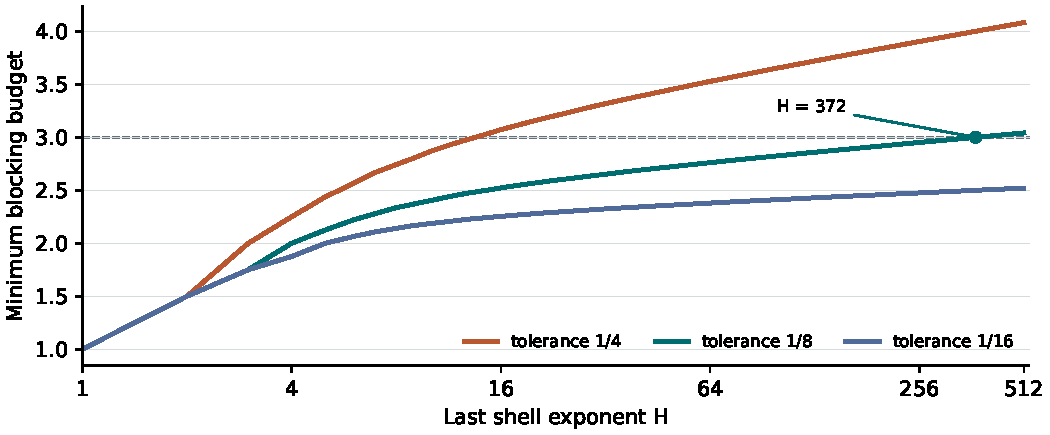
\includegraphics[width=.94\linewidth]{selection_budget.pdf}\\[-2pt]
{\small\itshape Minimum budget for blocking every dyadic shell through $H$.
The horizontal line marks the witness budget $B=3$.}\end{center}

\section{Recovering both arithmetic parameters from a finite signed zero list}
\label{sec:inverse}
The signed residues in the Lean proof retain surprisingly specific arithmetic
information. The earlier critical-line report \cite{priorzero} reconstructed the
modulus $q$ and auxiliary prime $d$ from their infinite sequence and asked for
a certified stopping rule with approximate data when both conductors are
unknown. We give such a rule in the parameter range of the lattice argument.
Only this section uses Dirichlet GRH as a premise.

\begin{theorem}\label{th:inverse}
Suppose $18480\mid q$, $d$ is prime and $d\equiv q/2-1\pmod q$.
In particular $d\equiv7\pmod8$, $(q,d)=1$, and $q\le2(d+1)$.
Set $h=\varphi(q)$, $\eta=(\cdot/d)$, and let $\chi^*$ denote the primitive
character inducing $\chi$. At $\rho=1/2+i\gamma$ the supplied ordinate weight is
\[
 m(\gamma)=h^{-1}\sum_{\chi\bmod q}
 \left(\operatorname{ord}_\rho L(s,\chi^*)-
       \operatorname{ord}_\rho L(s,\chi^*\eta)\right).
\]
Knowing the signed list through a sufficiently high finite height determines
$q,d$. The algorithm needs no prior numerical upper bound on either.
For approximate input it accepts enclosures for the finite sums it uses.
With complete lists and arbitrarily refinable certified errors it terminates.
For exact input a sufficient height is $O(d^2\log^3(2d))$ with an absolute
implied constant. This is a height estimate, independent of the cost of
computing or certifying the input lists.
\end{theorem}

\subsection*{Two terms in the explicit formula}
Write $\widehat g(\gamma)=\int g(t)e^{i\gamma t}\,dt$. For real compactly
supported test functions, the character-averaged Guinand--Weil formula takes
the form
\begin{align*}
 -\sum_\gamma m(\gamma)\widehat g(\gamma)
  ={}& (\log d)g(0)-\frac2h\int g(t)\cosh(t/2)\,dt\\
 &+\sum_{n=p^k}\frac{\log p}{\sqrt n}\,A(n)
                 [g(\log n)+g(-\log n)] .
\end{align*}
For $Q=p^{v_p(q)}$ the coefficient is
$A(n)=(1-\eta(n))\mathbf1_{n\equiv1\bmod(q/Q)}/\varphi(Q)$.
Here and below the sum over $n=p^k$ has $k\ge1$.
To check the identity, the primitive conductors in each pair are $f$ and $fd$,
so the signed minus sign yields $+\log d$ at the origin. Half of the characters
have each parity and twisting interchanges the two, canceling the gamma terms.
Only the untwisted family has the completed zeta poles. At $p\mid q$,
primitivization contributes only when the $p$-component is principal;
orthogonality over $q/Q$ gives the stated coefficient. Complex conjugates
occur in pairs. These are the terms of the classical explicit formula
\cite{chirre,booker}, specialized to the residue difference in
\path{New/Reduction/Zeros/PrimeError.lean}.

Consequently if $g$ kills the $\cosh(t/2)$ integral, has value one at $u$,
and its support isolates $u$, the measured quantity is $J(u)$, where
\[
 J(0)=\log d,\qquad J(\log p)=
 \frac{2\log p}{\sqrt p}\mathbf1_{q\mid p-1}
 \quad\text{for }p\nmid qd,\quad\eta(p)=-1 .
\]
The origin and prime identities alone would only give an asymptotic
reconstruction. To certify a finite stopping time we need to estimate the
unseen zero contribution before knowing the conductors.

\subsection*{A bound containing the unknown on both sides}
For a primitive character of conductor $f$, parity $a\in\{0,1\}$, let $B_f$
denote the sum of $(1+\gamma^2)^{-1}$ over its nontrivial zeros, including
multiplicity. Hadamard factorization and the functional equation give at $s=2$
\[
 \sum_\gamma\frac{3/2}{9/4+\gamma^2}=
 \Re\frac{L'}L(2)+\tfrac12\log(f/\pi)+\tfrac12\psi(1+a/2)
 +\tfrac32\mathbf1_{f=1}.
\]
This is the real logarithmic derivative of the completed entire function, with
$s(s-1)$ included for zeta \cite{lls}. GRH gives the indicated denominators.
Multiplying the summand by $3/2$ majorizes $(1+\gamma^2)^{-1}$.
For $f>1$, $|L'/L(2)|\le\sum_{n\ge2}(\log n)/n^2<1$ (isolate 2 and 3,
integrate from 3). For $f=1$ the logarithmic derivative is negative.
Since $\psi(1+a/2)\le\psi(2)<\log\pi$, in both cases
$B_f\le\tfrac34\log f+\tfrac94$.
Averaging absolute values before taking the signed difference yields
\[
 W:=\sum_\gamma\frac{|m(\gamma)|}{1+\gamma^2}
 \le \tfrac32\log q+\tfrac34\log d+\tfrac92
 \le \tfrac94\log d+7 ,
\]
using $q\le3d$. The dependence on $\log d$ here can be absorbed into the
origin measurement.

For any chosen test $g$, suppose $A$ bounds
$\sup_{|\gamma|>T}(1+\gamma^2)|\widehat g(\gamma)|$.
Let $[l,u]$ enclose the real part of the negative sum through height $T$.
The imaginary part of the exact full sum vanishes. For the origin probe put
$y=\log d$. Whenever $9A/4<1$, the arithmetic certificate is
\[
 \boxed{\quad \frac{l-7A}{1+9A/4}\ \le\ y\ \le \ \frac{u+7A}{1-9A/4}.\quad}
\]
Exponentiate with outward rounding. Stop the first stage when there is just
one admissible prime integer in the resulting interval. After that stage the
error for each new probe is at most $A(9\log d/4+7)$, independent of $q$.
A finite interval can likewise be certified by summing enclosures of
$m(\gamma)\widehat g(\gamma)$; omitted or uncertain entries require an enclosure
of their possible total contribution. Without such an input error guarantee a
list may omit a decisive term.

\subsection*{Two explicit probes}
A simple choice at location $v$ is the translate by $v$ of
\[
 g_a(t)=\frac{f_a''(t)-f_a(t)/4}{f_a''(0)-1/4},
 \qquad f_a(t)=\big(1-(t/a)^2\big)_+^8 .
\]
It equals one at its center and kills both $e^{t/2}$ and $e^{-t/2}$ by
integration by parts. Use $a=1/2$ at zero, or $a=1/[3(p+1)]$ at $\log p$;
the distance to the nearest other logarithm of a positive integer is at least
$\log(1+1/p)\ge1/(p+1)$. Four integrations by parts permit
$A=\|g_a^{(4)}\|_1(1+T^2)/T^4$. The accompanying script bounds this norm
term by term with rational arithmetic.

For the sharper height estimate, take $b=1/6$ at zero and
$b=1/[10(p+1)]$ at $\log p$. Set $k=\lfloor bT/2\rfloor\ge4$.
Convolve the uniform probability density on $[-b/k,b/k]$ with itself $k$
times and divide by its value at zero to obtain $w$. It is symmetric and
unimodal (averaging any symmetric unimodal density on a centered interval
preserves this property). Before normalization its maximum is at least $1/(2b)$
by total mass and support. Define
\[
 g(t)=w(t-v)-\frac{w(t-v-2b)+w(t-v+2b)}{2\cosh b}.
\]
The support lies within $3b$ of the center, $g(v)=1$, and translation of
$e^{\pm t/2}$ by $\pm2b$ cancels its integral. The Fourier transform of the
unnormalized $w$ is $\operatorname{sinc}(b\gamma/k)^k$, where
$\operatorname{sinc}(x)=\sin(x)/x$. For $|\gamma|>T$ the absolute
value is at most $2^{-k}(T/|\gamma|)^k$. The translation multiplier is at
most two, so we can use
\[
 A=4b(1+T^2)\,2^{-\lfloor bT/2\rfloor}.
\]
The probes have sufficient differentiability for the explicit formula:
convolution with smooth approximate identities gives the same identity in
the limit, with spectral domination by a multiple of $(1+\gamma^2)^{-1}$.
Increasing $T$ and refining enclosures therefore certifies $d$ at the
origin. One can, for example, choose $T$ dyadically and refine the finite
sum enclosure to width $1/T^2$ or smaller; adaptive refinement to arbitrary
accuracy at each trial also works. For exact data $T=O(\log(2d))$ suffices at
the origin since adjacent integer logarithms near $d$ are separated by
$\gg1/d$. This last scale estimate assumes exact finite sums.

\subsection*{Separating the finitely many moduli}
Form $M=2(d+1)$. The remaining candidates are the divisors $q$ of $M$
with $18480\mid q$ and $M/q$ odd. For two distinct candidates $q_1<q_2$,
there is a unit $u\bmod M$ congruent to one modulo $q_1$ and different
from one modulo $q_2$. Indeed choose a prime $\ell$ with
$v_\ell(q_1)<v_\ell(q_2)$. Prescribe the residue $1+\ell^{v_\ell(q_1)}$
modulo the full $\ell$-power in $M$, and one at all other prime powers.
If $v_\ell(q_1)=0$, this residue is two and $\ell$ is odd. Now require
$p\equiv u\bmod M$ and $\eta(p)=-1$. These conditions specify one coset of
index $2\varphi(M)$ modulo $Md$, since $(M,d)=1$. Dirichlet's theorem
gives a prime in this coset, and a search with integer tests finds one.
The two possible values of $J(\log p)$ are separated by $2\log p/\sqrt p$.
A certified interval excluding one value eliminates a candidate. Continuing
until only one remains proves finite recovery.

Lamzouri--Li--Soundararajan's Theorem 1.4 bounds the least prime in a coset
of index $I>1$ modulo $Q\ge20000$ by $O(I^2\log^2 Q)$ under Dirichlet GRH
\cite{lls}. Their explicit alternatives are $p\le10^9$ or
$p\le((I-1)\log Q+3(I+1)+\tfrac52(\log\log Q)^2)^2$. Here $I\le 2M$ and $Q=Md$, so each
witness can be taken $p\ll d^2\log^2(2d)$. For a sufficiently large absolute
constant, $T$ of order $p\log(2pd)$ makes the spline tail times $W$ less than
half the two-value separation. All witnesses use the same spectral list, so
the maximum of these heights proves the claimed bound.
\hfill$\square$

\paragraph{An arithmetic example.}
Take $d=109909799$. Sixteen candidate moduli survive the divisor tests. Even
knowing the totient would leave the pair $1127280,1201200$ at totient
$230400$. The prime $34945681$ is a quadratic nonresidue modulo $d$, and
$\gcd(p-1,2(d+1))=1127280$; its jump distinguishes the two. At $T=768$ the
spline at the origin has a tail below $1.045\cdot10^{-12}$ for this actual
$d$. At $T=6\cdot10^{10}$ the witness probe has a tail below
$5.220\cdot10^{-11}$, against a jump greater than $0.005875$.
The script checks primes, characters, candidate enumeration and tail
arithmetic. These are calculations on known parameters; an observed
spectral list of these heights was not computed.

\section{An optimal test for symmetric powers of an elliptic curve}
\label{sec:sym}
Fix a non-CM elliptic curve $E/\mathbb Q$ and an integer $d\ge1$.
Write $L_j(s)=L(s,\mathrm{Sym}^j E)$ in unitary normalization
(the center is $1/2$), and put $L_0=\zeta$.
For each good prime $p$, let $2\cos\theta_p=(p+1-\#E(\mathbb F_p))/\sqrt p$
with $0\le\theta_p\le\pi$. Define $V_0=1$, $V_1=z$ and
$V_{j+1}=zV_j-V_{j-1}$. Thus $V_j(2\cos\theta)=
\sin((j+1)\theta)/\sin\theta$, with endpoint values given by continuity.

\paragraph{An extremal polynomial.}
For a nonzero polynomial $f\ge0$ on $[-2,2]$ of degree at most $2d$,
write $f=\sum_{j=0}^{2d} a_j V_j$. The largest possible ratio $a_1/a_0$ is
\[
 u=2\cos\frac{\pi}{d+2}.
\]
The unique optimizer up to positive scale is
\[
 f_d(z)=\left(\sum_{j=0}^d V_j(u)V_j(z)\right)^2 .
\]
Every coefficient $a_0,\ldots,a_{2d}$ of this optimizer is strictly positive.
The ratio measures the coefficient of the ordinary trace when the mean
of the test is fixed. Other objectives, such as minimizing sample variance,
give different optimization problems.

\emph{Proof.}
The $V_j$ are orthonormal for
$d\mu(z)=\sqrt{4-z^2}\,dz/(2\pi)$ by sine orthogonality.
Write $\theta_i=i\pi/(d+2)$, $z_i=2\cos\theta_i$ and
$w_i=2\sin^2\theta_i/(d+2)$, for $1\le i\le d+1$.
The rule $\int g\,d\mu=\sum_i w_i g(z_i)$ holds through degree $2d+1$.
Indeed, divide $g$ by $V_{d+1}$, which vanishes at all nodes. The quotient
has degree at most $d$, so the integral of the multiple of $V_{d+1}$
vanishes by orthogonality. Discrete sine orthogonality gives the formula for
the remainder. Now $a_1/a_0=\int zf\,d\mu/\int f\,d\mu$ is a weighted
average of the nodes, so it is at most $z_1=u$.
Equality forces $f$ to have a double zero at every other node, fixing its
shape up to scale. Discrete sine orthogonality gives
$\sum_{j=0}^d V_j(z_1)V_j(z_i)=0$ for $i>1$, so $f_d$ attains equality.
Each $V_j(u)$ is positive for $0\le j\le d$. The product rule
$V_j V_k=V_{j+k}+V_{j+k-2}+\cdots+V_{|j-k|}$ follows from the sine formula.
For each $0\le m\le2d$, some $j,k\le d$ have $j+k=m$, so $a_m>0$.
\hfill$\square$

\paragraph{A fourth-power criterion.}
Use the extremizer just obtained and form the positive sum
\[
 S_f(x)=\sum_{\substack{p^k\le x,\ k\ge1\\p\ {\rm good}}}
 (\log p)\, f(2\cos(k\theta_p))\left(\frac1{p^k}-\frac1x\right).
\]
Write $L_j^{(S)}$ for the Euler product with bad primes omitted and set
\[
 D(s)=-\sum_{j=0}^{2d}a_j\frac{(L_j^{(S)})'}{L_j^{(S)}}(s),\qquad
 C=\lim_{s\to1}\left(D(s)-\frac{a_0}{s-1}\right)-a_0,\qquad
 R_f(x)=S_f(x)-a_0\log x-C .
\]
Bad Euler factors have normalized inverse roots of modulus at most one,
so their removal introduces no zeros in $\Re s>0$. For fixed $j\ge1$,
cuspidal automorphy, entireness of the completed function and functional
equation are available by modularity and Newton--Thorne, Theorem A and
Corollary B (\emph{Publ. Math. IH\'ES} 134, 2021,
\href{https://doi.org/10.1007/s10240-021-00126-4}{doi:10.1007/s10240-021-00126-4}).
We use Jacquet and Shalika's nonvanishing theorem on $\Re s=1$
(\emph{A non-vanishing theorem for zeta functions of $\mathrm{GL}_n$},
\emph{Invent. Math.} 38 (1976), 1--16). In particular the displayed limit exists.

\textbf{Theorem.}
All nontrivial zeros of $L_0,\ldots,L_{2d}$ have real part $1/2$
if and only if, for each $\epsilon>0$, there exists $B_\epsilon>0$ with
\[
 R_f(n^4)\le B_\epsilon n^{-2+4\epsilon}
 \qquad\hbox{for all sufficiently large integers }n.
\]
Here $E$ and $d$ are fixed. The theorem yields a single positive prime
sum for a finite family of conjectures. Under the premise of the question,
the $j=0$ member is already supplied.

\emph{Interpolation.}
In $t=1/x$, the function $S_f(1/t)$ is convex. Each summand is a
nonnegative coefficient times $(p^{-k}-t)_+$. Between
$t_-=(n+1)^{-4}$ and $t_+=n^{-4}$ it is bounded by its secant.
The secant of $-a_0\log t$ exceeds that function by at most
$a_0(t_+-t_-)^2/(8t_-^2)=O_d(n^{-2})$, by the interpolation
remainder and the second derivative $a_0/t^2$. Since $x\asymp n^4$,
the sample bounds imply $R_f(x)\le B'_\epsilon x^{-1/2+\epsilon}$.
This argument accounts for the fourth powers and the sign of the test.

\emph{Zeros from the upper bound.}
In $\Re s>1$ termwise integration gives
\[
 H(s):=\int_1^\infty R_f(x)x^{-s}\,dx
  =\frac{D(s)}{s(s-1)}-\frac{a_0}{(s-1)^2}-\frac C{s-1}.
\]
Indeed $V_j(2\cos(k\theta_p))$ is the trace of the $k$th power of
the normalized Frobenius in $\mathrm{Sym}^j$. The definition of $C$
removes the singularity at $1$. At a zero $\rho$ in the open critical strip,
the residue is
\[
 \frac{\sum_j a_j\,\mathrm{ord}_{\rho}L_j}{\rho(1-\rho)}.
\]
It is positive at every real zero and nonzero at every nonreal zero,
including a zero shared by several factors.
For $\beta=1/2+\epsilon<1$, take the eventually nonnegative function
$B'_\epsilon x^{\beta-1}-R_f(x)$. Changing it on a compact interval
affects its transform by an entire function. If the Mellin integral of
this function has abscissa of convergence $\sigma_c>\beta$, Landau's
theorem forces a singularity there. The continued transform is meromorphic
with at most simple poles there, and a real pole has negative residue
by the displayed formula. This is impossible for an integral of a
nonnegative function as $s\downarrow\sigma_c$.
Consequently $H$ is holomorphic for $\Re s>\beta$. Letting
$\epsilon\downarrow0$ and using the functional equations proves the claim.
This argument allows arbitrary orders at the central point.

\emph{The reverse implication.}
Assume the stated zero location and fix $0<\epsilon<1/2$.
Invert $D(s)/(s(s-1))$ on $\Re s=2$ against $x^{s-1}$.
The inverse of each prime-power term is $(p^{-k}-x^{-1})_+$.
Shift the line to $\Re s=1/2+\epsilon$. The double pole at $1$
contributes $a_0\log x+C$. For clarity, the usual justification of
the shift uses the fixed-degree unitary $L$-functions' order-one Hadamard
products, their gamma factors and the local zero count
$N(T+1)-N(T)=O_{E,d}(\log(2+T))$.
Subtracting the logarithmic derivative at $2+it$ from that at
$\sigma+it$ gives an absolutely convergent zero sum: the zeros with
$|\Im\rho-t|\le1$ contribute $O_{E,d,\epsilon}(\log(2+|t|))$ since
$|\sigma+it-\rho|\ge\epsilon$. More distant zeros contribute the same
bound by summing unit bands with weights $O((1+|t-\Im\rho|)^{-2})$.
Stirling's formula bounds the gamma terms. Thus $D(\sigma+it)$ is
$O_{E,d,\epsilon}(\log(2+|t|))$ uniformly on the shifted strip for
$|t|\ge2$. The quadratic denominator gives absolute convergence on the
new line and vanishing horizontal integrals. This gives the stronger
two-sided bound $|R_f(x)|\ll_{E,d,\epsilon} x^{-1/2+\epsilon}$.

\paragraph{The first four symmetric powers.}
For $d=2$, $u=\sqrt2$ and $f_2(z)=(z^2+\sqrt2 z)^2$.
Its character coefficients are $(4,4\sqrt2,5,2\sqrt2,1)$.
This gives an explicit target for an arithmetic upper bound at $x=n^4$.
The determinant estimates in the repository count congruence classes and
quadratic characters. A corresponding divisibility or height estimate
with these elliptic Frobenius weights is an additional arithmetic input.
The extremal problem and the sparse criterion are solved here. The bound
for this curve, and hence symmetric-power GRH, remains open in this analysis.

For the curve $y^2+y=x^3-x$, the discriminant is $37$ and
$j=48^3/37$ is nonintegral, which excludes CM. The accompanying
sample calculation counts points at every good prime up to $10^4$
and includes each admissible prime power. It gives
$S_f(16)=1.17616326$ and $S_f(10^4)=19.38460159$.
The table also gives consecutive differences of $S_f(x)-4\log x$,
in which the unknown additive constant cancels. These values illustrate
the observable at finite $x$.

\paragraph{How well can congruence weights approximate this test?}
For any fixed modulus $q$ and real function $g$ on its unit classes, write
$\pi_S(X)$ for the number of good primes $p\le X$ coprime to $q$.
The squared error for the local observable in the preceding example obeys
\[
 \lim_{X\to\infty}\frac{1}{\pi_S(X)}
 \sum_{\substack{p\le X\ {\rm good}\\p\nmid q}}
 \bigl(f_2(2\cos\theta_p)-g(p\bmod q)\bigr)^2
 =
 66+\frac1{\varphi(q)}\sum_{b\in(\mathbb Z/q\mathbb Z)^\times}
 (4-g(b))^2 .
\]
Indeed, in each unit residue class the average of
$V_j(2\cos\theta_p)$ tends to zero for $1\le j\le8$. Expand the class
indicator in Dirichlet characters and apply the prime number theorem to
the standard $L$-functions of $\mathrm{Sym}^j E$ twisted by these characters.
Each twist is cuspidal of degree $j+1>1$. Its standard $L$-function is
holomorphic and nonzero on $\Re s=1$, and its normalized prime-power traces
are bounded by $j+1$. These facts give the prime number theorem for the
trace by the usual Tauberian argument (add a sufficiently large constant
multiple of the zeta logarithmic derivative to bound the real and imaginary
coefficients by nonnegative ones, then subtract the ordinary prime number
theorem). Prime powers of exponent at least two cost $o(X)$ in the
log-weighted sum. Partial summation removes the logarithm.
Consequently the required average on class $b$ is its semicircle integral.
Orthonormality gives the squared fluctuation
$(4\sqrt2)^2+5^2+(2\sqrt2)^2+1^2=66$.
This quantifies precisely which local information survives every fixed
congruence test. It leaves open cancellation in a smoothed sum and the use
of moduli growing with the cutoff.


\clearpage
\section{Verification and further research}
For the torsion theorem, \path{check_minimax.py} enumerates all multisets of up to $e_h$ roots in eight small cyclotomic shells. It computes each valuation directly from the order of the difference of the exponents, before comparing the maximum over layouts to Theorem~\ref{th:cost}. The 14,872 layouts include repeated roots, empty layouts and full shells. Rounding arbitrary roots to the shell and reducing arbitrary packets to these layouts are proved in Section~\ref{sec:exact}. A second check tests the strict tolerance boundary at 12,640 triples $(p,B_*,\epsilon)$, counting repeated rational representations as separate test cases. The large-shell example uses exact integer comparisons.

For the inverse problem, \path{check_recovery.py} verifies the distinguishing prime and rational enclosures for the two truncation estimates. For the elliptic test, \path{elliptic_samples.py} produces the finite table from point counts; the logarithmic sums use floating-point arithmetic. Source identifiers, reproduction commands and outputs accompany the note. The two resolved questions were posed in the cited ProveIt reports. We have not established independent publication priority for the resulting theorems.

\subsection*{Questions left by the proofs}
\begin{enumerate}
\item For a fixed ramified field $K$, determine the exact shell budget as a function of $K\cap\mathbb Q_p(\zeta_{p^h})$ and the admissible coefficient valuations. The unrestricted construction uses individually chosen conjugates; the unramified case is exact at cost $H$.
\item For several coordinates, determine whether the leading exponential constant is achieved by a one-variable obstruction. Sequential substitution gives upper bounds, but it can spend the same tolerance at successive coordinates.
\item How low can the height needed to recover $(q,d)$ be? The upper bound here narrows a test around $\log p$ to isolate a single atom. Probes designed to distinguish two entire arithmetic signatures could use more of the prime data at one time.
\item Can a height or divisibility argument produce the elliptic upper bound in Section~\ref{sec:sym}, even for $y^2+y=x^3-x$ and $d=1$? For a fixed modulus, the exact variance calculation illustrates which part of the local data a proposed comparison must accommodate.
\end{enumerate}

\begin{thebibliography}{9}\small\raggedright
\bibitem{repo} L. Sernau and collaborators, \emph{GRH for Dirichlet $L$-functions, in Lean 4}, after L. Alp\"oge with Claude. \ghlink{grh/GUIDE.md}{Guide}, \ghlink{grh/src/Statements.lean}{public types}, \ghlink{grh/src/Main.lean}{exports}, \ghlink{grh/README.md}{verification and dependencies}.
\bibitem{priortorsion} V. Reshetnikov, ProveIt incoming reports. \href{https://github.com/VladimirReshetnikov/ProveIt/blob/6fe2c1bd450aa7f19eab17fb9a6e76170b4fce00/docs/incoming/grh_quantitative_twists_2026-11-25.zip}{\emph{Polynomial Order-Exponent Bounds for Simultaneous $p$-adic Twisting}}, question (ii), p.\ 10. The formulation with witnesses and total positive excess is in the companion archive \href{https://github.com/VladimirReshetnikov/ProveIt/blob/6fe2c1bd450aa7f19eab17fb9a6e76170b4fce00/docs/incoming/grh_method_transfers_2026-11-25(1).zip}{\texttt{grh\_method\_transfers\_2026-11-25(1).zip}}, \path{sections/torsion_transfer.tex}.
\bibitem{bhargava} M. Bhargava, \href{https://www.sciencedirect.com/science/article/pii/S0022314X9892220X}{Generalized factorials and fixed divisors over subsets of a Dedekind domain}, \emph{J. Number Theory} 72 (1998), 67--75.
\bibitem{priorzero} ProveIt, \href{https://github.com/VladimirReshetnikov/ProveIt/blob/6fe2c1bd450aa7f19eab17fb9a6e76170b4fce00/docs/incoming/dirichlet-grh-research.zip}{\emph{Beyond Dirichlet GRH}}, critical-line paper, \path{cusp.tex}, \path{band.tex} and research question 3 in \path{critical-line.tex}.
\bibitem{chirre} A. Chirre, V. J. Pereira J\'unior and D. de Laat, \href{https://doi.org/10.1090/mcom/3638}{Primes in arithmetic progressions and semidefinite programming}, \emph{Math. Comp.} 90 (2021), \S2.
\bibitem{booker} A. Booker, \href{https://doi.org/10.1007/s00208-015-1178-z}{$L$-functions as distributions}, \emph{Math. Ann.} 363 (2015), 423--454.
\bibitem{lls} Y. Lamzouri, X. Li and K. Soundararajan, \href{https://arxiv.org/abs/1309.3595}{Conditional bounds for the least quadratic non-residue and related problems}, \emph{Math. Comp.} 84 (2015), 2391--2412, \S2 and Theorem 1.4; \href{https://doi.org/10.1090/mcom/3261}{corrigendum}, 86 (2017), 2551--2554.
\end{thebibliography}
\end{document}
